\documentclass[12pt,a4paper]{article}

\usepackage{amsmath}
\usepackage{amsfonts}
\usepackage{amssymb}
\usepackage{graphicx}
\usepackage{graphics}
\usepackage{algorithm}
\usepackage{algorithmic}
\usepackage{etoolbox}\AtBeginEnvironment{algorithmic}{\small}
\usepackage{caption}
\usepackage{pythonhighlight}
\captionsetup{font=footnotesize}
\setlength{\parindent}{0pt}

\begin{document}

\Large
\begin{center}
Where Steaks Meet Statistics: Modeling Inventory Demand as a Finite-Horizon Markov Decision Process
\hspace{20pt}

\large
Alex Huml$^1$, Carter Hall$^1$, Thomas Bridges$^1$, Ian Wilson$^1$\\

\hspace{10pt}

\small  
$^1$ Department of Statistics and Operations Research, University of North Carolina at Chapel Hill\\

\end{center}

\hrulefill
\normalsize

\section{Abstract}

This report presents a practical intersection of statistics, economics, and industry by modeling inventory decisions for a local steakhouse, Stoney River Steakhouse and Grill. After an arduous process of converting physical data into a digital format, recent sales records for four main varieties of steak were utilized as respective foundations for finite-horizon Markov Decision Processes (MDPs). Prices were transformed according to the inflation rate, such that future decisions would account for economic inflation (FRED, 2022). The resulting optimal policies are reflective of potential ordering practices for the business, as they aspire to effectively meet customer demands, now and in the future.

\section{Background}

In aspiring to model these inventory decisions for Stoney River through an MDP, careful assumptions and observations had to first be made to ensure the relevance of any concluded results. At this location, the restaurant orders from tenderloin, bone-in ribeye, or ``cowboy," strip, or boneless ribeye loins/steaks. Additionally, Stoney River orders ground chuck meat as well, though as this is sometimes used in-place of other steaks as ``side items," the modeling process ignores these orders and considers the four aforementioned categories.
\\

\subsection{Important Observations}

For each type of loin, of major importance is the amount Stoney River is capable of storing at any one time; there can be 84 tenderloins, 9 cowboy loins, 12 strip loins, and 24 ribeye loins in Stoney River's storage. Such large figures allowed for the removal of any spoilage considerations, as demand for the steaks is fast enough in comparison such that meat seldom, if at all, spoils. As for the MDPs, these values, when converted to pounds, were able to serve as maxima for each process' respective state space. 
\\

Another complication arises from the explicit measurements of steaks as ordered by the customer; to circumnavigate this, all data was converted into pounds such that the end-result could be interpreted into pounds and partitioned into individual orders as the restaurant desires. For context, the following information is given for each loin:
\\

$ \bullet \text{ Strip: 5 loins per case, at an average of 13 lbs per loin}  $

$ \bullet \text{ Cowboy: 3 loins per case, at an average of 18 lbs per loin}  $

$ \bullet \text{ Ribeye: 4 loins per case, at an average of 15 lbs per loin}  $

$ \bullet \text{ Tenderloin: 12 loins per case, at an average of 7 lbs per loin}  $
\\

It should be noted that, as not all cows are created equal (differing in size by the season), formatting of the results in this manner allows for a better frame of reference when the restaurant places order(s) from their supplier(s).

\subsection{Assumptions}

Before presenting the framework behind the MDPs, a few important assumptions and considerations should be presented, namely:

\begin{enumerate}
\item The restaurant previously sold a 12-ounce filet, but has since removed the option from the menu, leaving an already existent option of ordering a 10-ounce instead. To account for the same demand, the assumption is made that customers who previously ordered the 12-ounce filet will now order its smaller counterpart.

\item Some steaks will inevitably not be to customers' satisfactions, and will therefore be thrown out. However, as the meat was utilized by the kitchen, the demand is recognizable from the restaurant's perspective, and so inflated demands due to mis-cooked steaks are assumed to be negligible.

\item When entering the data into Excel spreadsheets, an issue arose with respect to the classification of orders based on the week of the year. The assumption of every month having four weeks was made, wherein this last week could have any additional days that would otherwise constitute a fifth. Hence, ``4.1" in the Excel documents, for example, corresponds directly to the first week of April.

\item In actuality, the restaurant could order anywhere from one to four times per week. Given that this is unpredictable from the perspective of the authors (and a Poisson process in general that we have no data to quantify), the assumption is made that prices do not change mid-week, hence the data is recognized as week-long totals.

\item As no spoilage is assumed due to capacity restrictions, salvage costs are considered to be negligible.

\item To discretize the normal distributions associated with demand patterns for each type of steak, Equation \ref{1} demonstrates the assumption for an arbitrary normal random variable, $X$. Furthermore, the normal distributions explained in Section 2.3 are assumed to be independent from one another, as there is no real and effective manner in which quantifying how an order of one steak could detract from the order totals of another.
\end{enumerate}

\begin{equation} \label{1}
F(x) = P(X = \lceil x \rceil) - P(X = \lfloor x \rfloor)
\end{equation}


\subsection{Creating Demand Probability Distributions}

Unfortunately, Stoney River was not able to supply week-long data as desired, but instead gave year-long totals for the amount of each steak sold. This forced the creation of an accurate probability distribution that did not rely on the fitting of a model to data points. After consultation with the restaurant's general manager, the conclusion was reached to use approximation to a normal distribution for each steak type. This decision was fortified due to assurance that the week-to-week demand was not a volatile figure, with the exception of holiday weeks or unusual ``down periods." 
\\

As the order data was in-hand, the standard deviation of the pounds of loins ordered per week was derived and used as a proxy for the standard deviation of any demand distribution. However, because orders are placed multiple times per week and not every pound ordered goes into making the steaks whose demands are being modeled, only half of the standard deviation was elected to be used to account for such a trend. Therefore, the following probability distributions were derived for each steak:
\\

$ \bullet \text{ Strip: } \mathcal{N}(112, 43)  $

$ \bullet \text{ Cowboy: } \mathcal{N}(54, 26)  $

$ \bullet \text{ Ribeye: } \mathcal{N}(119, 54)  $

$ \bullet \text{ Tenderloin: } \mathcal{N}(188, 89)  $
\\

\subsection{Prices}

As is the case with food, two prices are of importance: order price and selling price. The process to create the figure for the selling price was rather straightforward; as Stoney River sells different sized entrees of the same cut of beef (i.e. 10 and 16-ounce strips), computing a weighted average of the prices based on how much each steak was sold, in relation to the total, led to a single number representing price per pound for each steak. 
\\

The purchase prices for each steak type are presented in Figure 1, with the price per pound for each steak in the caption.

To model expected prices, price data was adjusted according to the rate of inflation. For each steak type, a scatter-plot relating price by week was matched to changes in the inflation rate. Expert predictions for inflation rates for the rest of the year were consulted, though of major relevance is the Russia-Ukraine conflict that is driving inflation rates up in the short-term. Equation 2 represents the price at an epoch, $Pr(t)$, modeled for each steak type in terms of average price over 2021, $A$. 
Note that $A$ is given as follows for each steak type (all in USD) $\text{ Strip: } 8.96, \text{ Cowboy: } 11.32,$ $\text{Ribeye: } 12.68, \text{ Tenderloin: } 14.98.$
\\

\begin{equation} \label{2}
Pr(t) = A + (1 + \frac{0.05}{\sqrt{t} - 0.5}) 
\end{equation}

The evaluation behind this projection is that prices will decrease in the latter half of 2022, though remain higher than $A$. 

\newpage

\begin{figure}[H]
\centering
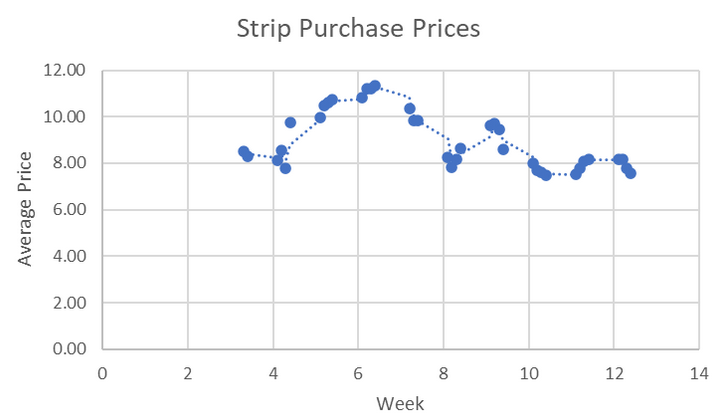
\includegraphics[scale=0.6]{./Figures/Figure1a.png}
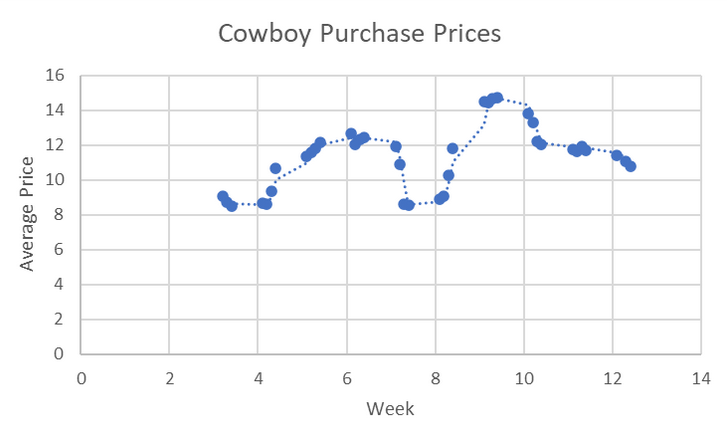
\includegraphics[scale=0.6]{./Figures/Figure1b.png}
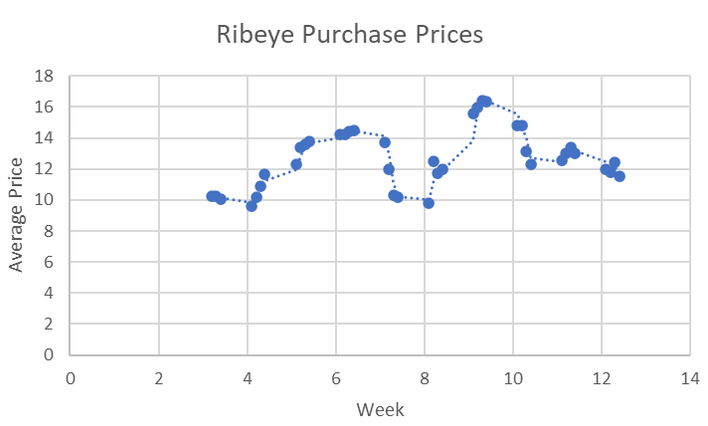
\includegraphics[scale=0.6]{./Figures/Figure1c.png}
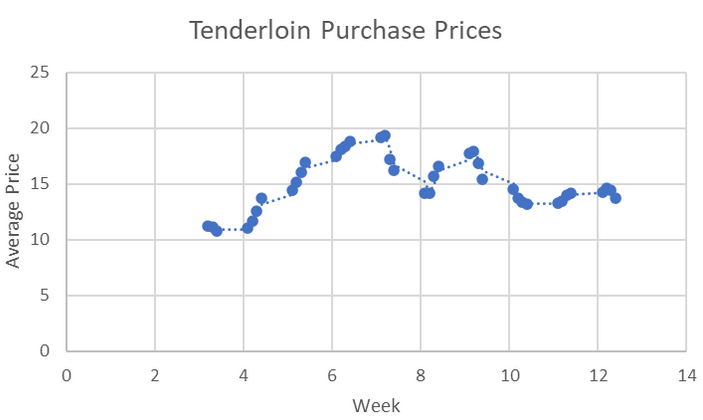
\includegraphics[scale=0.6]{./Figures/Figure1d.png}
\caption{Purchase prices for each steak, by week. The selling price, per pound, for each steak is as follows: \textit{Strip} = 44 USD, \textit{Cowboy} = 36 USD, \textit{Ribeye} = 48 USD, \textit{Tenderloin} = 75 USD.}
\end{figure}

\section{Setup of the MDPs}

As a summary of the presented background information, this section presents the information for the finite-horizon Markov Decision Processes, who in general reflect the 5-tuple

$$(T, S, A, p_{t}(s,a,j), r_{t}(s,a,j)) $$

where $T = \{1,2,...,32\}$ represents the set of decision epochs corresponding to each week, since the beginning of May. Note the selling prices from Figure 1 are given as $S_{p}$. To avoid redundancy in this report, let $s_{max}$ be the maximum state attainable for each steak type, given as:
\\

$ \bullet \text{ Strip: } 168  $

$ \bullet \text{ Cowboy: } 171  $

$ \bullet \text{ Ribeye: } 360  $

$ \bullet \text{ Tenderloin: } 588  $
\\

This gives the following for the state and action spaces $S$ and $A$, respectively,

$$\begin{cases}
S = \{0, 1, ..., s_{max} \} \\
A_{s} = \{0, 1, ..., s_{max} - s \} \forall s \in S \\
\end{cases}$$

Additionally, the reward and transition probability functions are qualitatively equivalent, and so they are given universally by Equations 3 and 4. Note $\text{CDF}$ represents the CDF of a normal distribution, using the normal distribution parameters presented in Section 2.3.

\small
\begin{equation} \label{3}
r_{t}(s,a,j) = \begin{cases} S_{p} *(s + a - j) * F(s + a - j) - a*Pr(t) & j \in [0,s+a] \\ S_{p} *(s + a) * (1 -  \text{CDF}(s + a)) - a*Pr(t) & \text{else} \end{cases} 
\end{equation}

\normalsize

\begin{equation} \label{4}
p_{t}(s,a,j) = \begin{cases} 0 & j > s + a \\ F(s + a - j) & 0 < j \leq s + a \\ 1 - \text{CDF}(s + a) & j = 0 \end{cases}
\end{equation}

\section{Results}

\section{Conclusion}

\newpage

\section{Literature Cited}

“Beef2022 Data - 2001-2021 Historical - 2023 Forecast - Price - Quote - Chart.” 
\textit{Beef - 2022 Data - 2001-2021 Historical - 2023 Forecast - Price - Quote - Chart}, https://tradingeconomics.com/commodity/beef. 
\\

“Prices - Inflation Forecast - OECD Data.” TheOECD,
https://data.oecd.org/
price/inflation-forecast.htm. 
\\

“10-Year Breakeven Inflation Rate.” FRED, 29 Apr. 2022, 

https://fred.stlouisfed.org/series/T10YIE. 
\\

“Consumer Price Index for All Urban Consumers: All Items in U.S. City Average.” FRED, 12 Apr. 2022, https://fred.stlouisfed.org/series/CPIAUCSL. 

\section{Appendix A: Python Code}

Stapled to this report will be a printout of the outputs, stored in Microsoft Excel. This appendix contains the relevant Python code, beginning on the following page. An entire repository containing this paper, code, and related output files can be found at the following link: 
https://github.com/halljc76/
STOR515FinalProj. 
\\

\textit{As efforts to implement concurrent programming via the \textbf{threading} package has been unsuccessful, an alternative measure was to open four separate kernels, copy the codebase file three times, and concurrently run each individual MDP in its own kernel. The class calls can be found in the linked repository above. This cuts the runtime in half on a normal laptop, from experimentation.}
\\
\newpage

\small 

\begin{python}
class WeLoveSteak:
    """Modeling the demand for delicious steaks as a finite-horizon Markov Decision Process."""
    def __init__(self, M, N, mu, sigma, sellPrice, priceyint, steakName):
        """Initialization Function.
        
        Parameters:
        M := Limit on storage capacity.
        N := Number of decision epochs.
        S := State Space. T := Epoch set.
        mu, sigma := Normal dist parameters.
        priceyint := P_0
        steakName := Name to pass into Excel writer.
        """
        self.M = M
        self.N = N
        self.S = set(range(self.M+1))
        self.T = set(range(1,self.N+1))
        self.mu = mu
        self.sigma = sigma
        self.sp = sellPrice
        self.priceyint = priceyint
        self.ustar, self.astar = self.optimality(steakName)
        self.storeResults(steakName)
        
    def A(self, s):
        '''Function representing action space.
        
        Parameters:
        s := State from state space S.
        '''
        return set(range(0,self.M - s + 1))
    def f(self, s):
        """Revenue generated from selling loins at sp/pound.
        
        Parameters:
        s := State indicating number of loins sold.
        """
        return self.sp * s
    def price(self, t):
        """Price for Strip Loin, adjusted for inflation via CPI metric.
        
        Parameters:
        t := Epoch in T
        """
        return self.priceyint * (1 + (0.0125 / (np.sqrt(t) - 0.5)))
    def CDF(self, s):
        """Function for discretized probability that uses the normal CDF.
        
        Parameters:
        s := State in S
        """
        return stats.NormalDist(self.mu, self.sigma).cdf(s)
    def pt(self, j, s, a):
        '''Transition probability function.
            
        Parameters:
        j,s := states in S
        a := action in A
        
        Returns:
        0 if j > s + a
        CDF(s + a - j) - CDF(s + a - j - 1) if 0 < j <= s + a
        1 - CDF(s + a) otherwise
        '''
        assert type(j) == type(s) == type(a) == type(3)
        return 0 if j > s + a else 
        ((self.CDF(s + a - j) - self.CDF(s + a - j - 1)) 
          if ((0 < j) and (j <= s + a)) 
          else (1 - self.CDF(s + a)))
    def rt(self, t, s, a = 0):
        """Reward function for the finite-horizon MDP setup.
        
        Parameters:
        t := Epoch in T
        s := State in S
        a := Action in A
        """
        if t == self.N:
            return 0
        
        return -a*self.price(t) + sum([self.CDF(k) - self.CDF(k - 1) * self.f(k) for k in range(s+a+1)]) + sum([self.CDF(s+a) * self.f(s+a) for k in range(s+a+1, self.M+1)])
    def optimalAction(self, d):
        '''Function to determine which action corresponds to optimal policy.
        
            Parameters
            ----------
            d: dict -> dictionary of (action, optimality eqn. value) 
        '''
        v = max(d.values())
        for k in d.keys():
            if d[k] == v:
                return k

        raise ValueError("Should never get here, but.")
    def optimality(self, steakName):
        '''Implements algorithm to find optimal policy via backward induction.'''
        t = len(self.T) # From 1 to N + 1, this returns N 
        ustar = np.zeros([len(self.S), t])
        astar = np.zeros([len(self.S), t])
        
        # BC computation -- u_{N+1}^{*} (s) = r_{N} s for all s in S
        for s in self.S:
            ustar[s,-1] = self.rt(t,s)
        
        while t != 1:
            print(steakName + ": " + str(t))
            t -= 1
            for s in self.S:
                l = dict()
                for a in self.A(s):
                    temp = self.rt(t,s,a) + sum([self.pt(j,s,a) * ustar[j,t] for j in self.S])
                    l[a] = l.get(a, 0) + temp
                ustar[s,t-1] = round(max(l.values()), 4) # Rounding this because of PDF output -- doesn't change answer
                astar[s,t-1]= self.optimalAction(l)
        
        ustar = self.getOptimalityTable(ustar)
        astar = self.getOptimalPolicy(astar)
        return ustar, astar
    def getOptimalPolicy(self, astar):
        '''Pretty-prints the optimal policy dataframe.'''
        return pd.DataFrame(astar, 
        columns = ['Week {}'.format(t) for t in 
                   range(1,self.N+1)], 
                   index   = ['State {}'.format(s) 
                   for s in range(0,len(self.S))])
    
    def getOptimalityTable(self, ustar):
        '''Pretty-prints the total expected reward dataframe.'''
        return pd.DataFrame(ustar, columns = 
        ['Week {}'.format(t) for t in range(1,self.N+1)], 
         index   = ['State {}'.format(s) 
         for s in range(0,len(self.S))])
    
    def storeResults(self, steakName):
        with pd.ExcelWriter("./MDPResults" + steakName + ".xlsx") as writer:
            self.astar.to_excel(writer, sheet_name="ExpReward", index=True)
            self.ustar.to_excel(writer, sheet_name="OptPolicy", index=True)
        return
\end{python}

\end{document}